\section{Vocoders}
\label{vocoders}
The interface with both the natural speech and the synthesized speech is the vocoder. 
%
In this section, the fundamentals of the vocoder are presented and a detailed description of the two vocoders compared in this project is given.

\subsection{Basics}
\label{vocoders_basics}
The human speech is produced by regulating the air from the lungs through the throat, mouth and nose. 
%
The airflow from the lungs is modulated at the larynx by the vocal folds, creating the main excitation for voiced speech. 
%
The airflow is then filter by the vocal tract, formed by the pharynx and the oral and nasal cavities, acting as an acoustic time-varying filter by adjusting the dimensions and volume of the pharynx and the oral cavity.

The main functions of the vocoder are translating from natural speech to spectral and excitation parameters and from these features to synthetic speech.
%
Thus, the vocoder should try to mimic the process involved in the human speech production.

As established in Section \ref{hmm_synthesis_parametrization}, the source-filter theory is a functional trade-off behaving quite well in statistical speech synthesis.
%
Hence, the basic vocoder could be the source-filter theory itself, modelling the source signal as a pulse train for voiced segments and white Gaussian noise for the unvoiced ones, i.e. impulse excitation vocoder.

The source-filter theory itself does not produce a high-quality synthetic speech.
%
The very simple excitation modelling cannot correctly model some of the speech sounds.
%
However, more complex vocoders as the compared in this project, GlottHMM and STRAIGHT, are also based on the source-filter theory, making the impulse excitation vocoder a standard to compare other vocoders with to test the quality.
%
Apart from its benchmark functions, this simple vocoder has been historically significant for the development of statistical speech synthesis.

Among the different types of existing vocoders, in the following sections the two compared in this project are explained.

\subsection{GlottHMM}
\label{vocoders_glott}
GlottHMM is a glottal source modelling vocoder.
%
The main characteristic of glottal source modelling vocoders is that they use estimated characteristics of the real glottal pulse in the determination of the exciting signal.
%
GlottHMM was proposed by Tuomo Raitio in \cite{TuomoMSc} and later improved \cite{raitio_tasl}.

The main idea in GlottHMM vocoder is to estimate the real glottal pulse signal and the real vocal tract filter associated with it.
%
To achieve that, a method called Iterative Adaptive Inverse Filtering (IAIF) is used \cite{alku1992glottal}.
%

The advantage of the proposed method is that real glottal pulses can be used as the excitation signal when synthesizing, therefore providing a more natural synthetic speech compared to pulse train excitation, making a quality improving.
%
Moreover, the glottal flow spectrum can be easily adapted or modified.

A highly detailed description of GlottHMM can be found in \cite{TuomoMSc} and \cite{manuMSc}.
%
In the next subsections an overview of the modules of GlottHMM is given, but it is not a deep description.

\subsubsection{Analysis}
\label{vocoders_glott_analysis}
During the analysis, GlottHMM first high-pass filters the speech signal from 70 Hz onwards.
%
Then, the speech signal is windowed into fixed length rectangular frames, from which the log energy is calculated as a feature parameter.

Secondly, the IAIF algorithm is applied to each frame resulting in the LPC representation of the vocal tract spectrum and the waveform representation of the voice source.
%
It calculates the LPC spectral envelope estimate of the voice source and along with the LPC estimate of the vocal tract is converted into a Line Spectral Frequency (LSF) representation \cite{manuMSc}.
%
The glottal waveform is used for the acquisition of the $F_{0}$ and the Harmonic-to-Noise Ratio (HNR) values for a predetermined number of frequency sub-bands.

The estimated glottal flow signal is used to produce the rest of the parameters. A voicing decision based on zero-crossings and low-band energy (less than 1 KHz) is made.
%
For voiced frames, the $F_{0}$ value is calculated with an autocorrelation method.
%
The HNR is calculated from the Fourier transform of the signal, evaluating the cepstrum of each frequency band.
%
For each frequency band, the degree of harmonicity is determined by the strength of the cepstral peak (defined by $F_{0}$) in ratio to the averaged value of other quefrencies of the cepstrum. 
%
For unvoiced frames, the $F_{0}$ and HNR values are set to zero.

\begin{figure}[!htb]
\begin{centering}
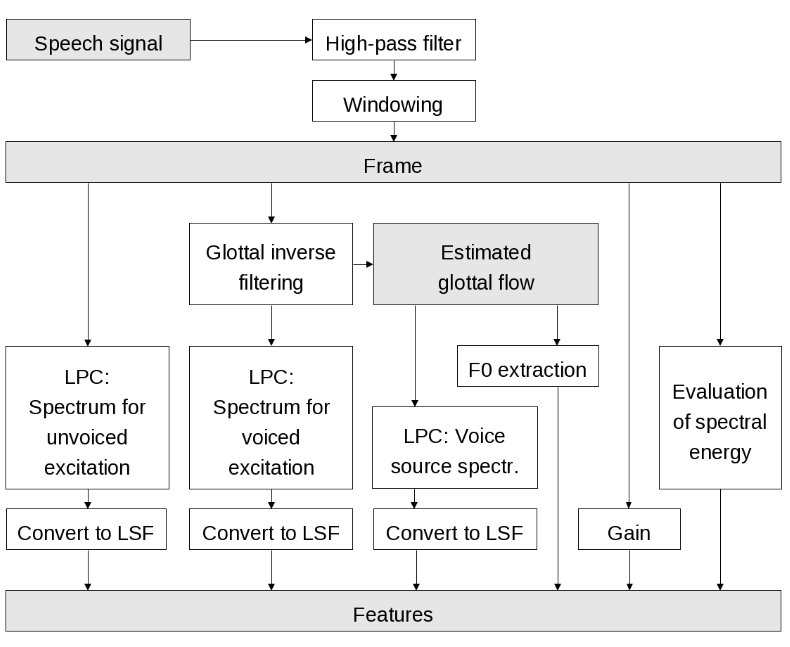
\includegraphics[width=0.7\textwidth]{images/glott_analysis.jpg}
\caption{Flow chart of the analysis made by GlottHMM \cite{TuomoMSc}}
\label{fig:glott_analysis}
\end{centering}
\end{figure}

The feature vector extracted from the analysis made by GlottHMM is composed of:

\begin{itemize}
	\item Excitation parameters: $F_{0}$, log energy, $m$ HNR sub-bands and $n$ order glottal source LSF
	\item Spectral parameters: $p$ order vocal tract LSF
\end{itemize}

Usually 5 HNR sub-bands are used and the orders of the glottal source and vocal tract LSFs are around 10-20 and 20-30 respectively.

\subsubsection{Synthesis}
\label{vocoders_glott_synthesis}
GlottHMM uses for the excitation generation a method based on the voiced/unvoiced decision in stead of using the traditional mixed excitation model for the excitation generation, as most of the state-of-the-art vocoders use. In Figure \ref{vocoders_glott_synthesis} the block diagram of the synthesis process of GlottHMM is shown.

\begin{figure}[!htb]
\begin{centering}
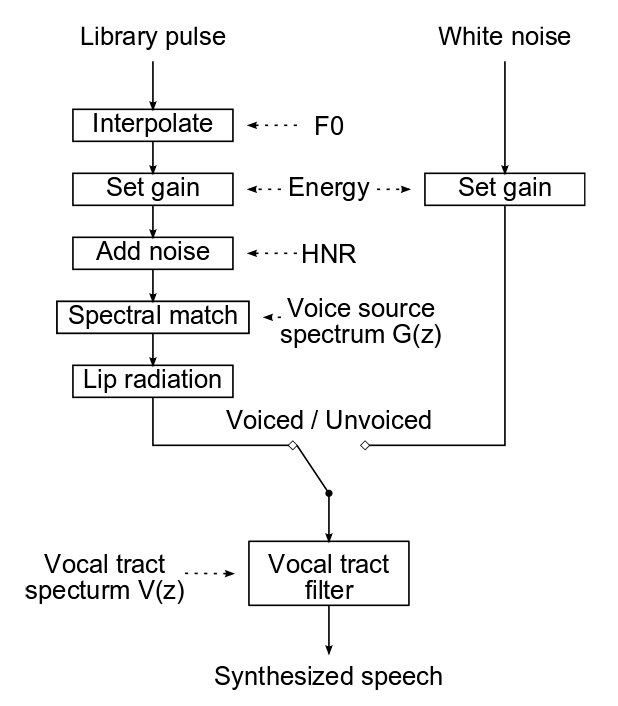
\includegraphics[width=0.6\textwidth]{images/glott_synthesis.jpg}
\caption{Synthesis block diagram of GlottHMM \cite{manuMSc}}
\label{fig:glott_synthesis}
\end{centering}
\end{figure}

For voiced frames, a fixed library pulse obtained by glottal inverse filtering a sustained vowel signal is interpolated to match the target $F_{0}$, using cubic spline interpolation, and its energy is set to match the target gain from the feature vector.

The next step is to conduct an HNR analysis similar to the one done in the analysis described in \ref{fig:glott_analysis}.
%
Noise is added to the real and imaginary parts of the Fast Fourier Transform (FFT) for every sub-band, according to the differences between the obtain and target HNR values, acting similar to the voiced excitation for voiced frames.

The spectrum of the library pulse is matched to the target glottal pulse in the feature vector.
%
LPC analysis is performed for the spectral matching, post-filtering with the target synthesis filter. Finally, the lip radiation effect is added by filtering it with a fixed differentiator.

In the case of unvoiced frames, the excitation is generated with white Gaussian noise whose gain is set by the energy parameter in the feature vector.

The excitation is combined in the time domain by overlap-adding target frames and the final synthetic signal is generated by filtering the excitation with the vocal tract filter from the vocal tract LSFs in the feature vector.

\subsubsection{GlottHMM with Pulse Library Technique}
\label{vocoders_glott_pulse_library}
In \cite{TuomoMSc} and \cite{manuMSc} the pulse library for GlottHMM is described.
%
This method was tested in the inital experiments to find out if it improves the quality over the single pulse excitation technique.

The results obtained with the pulse library method were clearly poorer than the ones using the single glottal pulse, therefore discarding the use of the pulse library.

\subsection{STRAIGHT}
\label{vocoders_straight}
STRAIGHT is a mixed multi-band excitation (MBE) vocoder.
%
MBE vocoders use additional parameters with the $F_{0}$ to generate an accurate excitation signal reducing buzziness.
%
The common characteristic in this kind of vocoders is that the parameters are extracted in a uniform way without case-specific adaptation.

STRAIGHT is the most established of the sophisticated vocoding methods.
%
It was proposed by Kawahara \cite{kawahara1997speech} and has gone through extensive research and development, as it can be seen in \cite{kawahara1999restructuring}, for example.

STRAIGHT was originally designed as a tool for speech transformation and accurate spectral envelope representation.
%
Its original parameters are represented as Fourier transform magnitudes and their correspondent aperiodicity measurements.
%
They cannot be used in HMM synthesis because of the high dimensionality. 
%
This issue is was overcome with the HMM-modified version of STRAIGHT proposed in \cite{heiga2007details}, representing the spectral envelope as mel-frequency cepstral coefficients and averaging the corresponding aperiodicity measurements over five frequency sub-bands.

A detailed description of STRAIGHT can be found in \cite{kawahara1997speech}, \cite{heiga2007details} and \cite{manuMSc}.

\subsubsection{Analysis}
\label{vocoders_straight_analysis}
STRAIGHT aims to an extraction of a smoothed spectral envelope, minimizing the effect of periodicity interference in the analysis frames, i.e. the STRAIGHT spectral envelope is essentially independent of the excitation.

To extract the spectral envelope the signal is windowed using two complementary $F_{0}$-adaptive windows with equivalent temporal and spectral solutions.
%
Then, the original and complimentary magnitude spectrograms are calculated using both windows' functions and combined into a final spectrogram.

This method introduces an over-smoothing problem.
% 
To solve it, the use of a quasi-optimal smoothing function is proposed.

The aperiodicity measurements estimate the amount of harmonic information in relation to non-harmonic information in the signal.
%
This is ideally done by warping each frame according to the phase of its fundamental component, making the warped signal to have a regular harmonic structure and calculating the ratios between lower and upper spectral envelopes.
%
The upper spectral envelopes connects the spectral peaks while the lower one does the same with the valleys.

However, ideal solutions are usually not feasible and actually the unwarped aperiodicity measures are obtained by performing a table lookup of the lower-upper ratio from a database of known aperiodicity measurements.
%
Then, its weighted average in relation to the speech power spectrum is calculated, resulting in the aperiodicity measurement.

To extract the fundamental frequency trajectory, STRAIGHT uses a specific pith extraction algorithm called Time-domain Excitation extractor using Minimum Pertubatin Operator (TEMPO) \cite{kawahara1999restructuring}, based on the concept of instantaneous frequency.

The instantaneous frequency is extracted by the means of an analyzing continuous wavelet transform, which has the smallest amount of AM and FM properties at the fundamental frequency.

The HMM-adapted version of STRAIGHT transforms the STRAIGHT spectrum into a mel-frequency cepstral representation for statistical modelling.
%
The aperiodicity measures are also represented in a compressed form.

The feature vector obtained with STRAIGHT consists of:

\begin{itemize}
	\item Excitation parameters: $F_{0}$ and 5 order aperiodicity measure
	\item $p$ order STRAIGHT Mel-Frequency Cepstral Coefficient (MFCC)
\end{itemize}

\subsubsection{Synthesis}
\label{vocoders_straight_synthesis}
STRAIGHT synthesis is carried out in a frame-by-frame basis by creating a mixed excitation signal of the length of two pulse periods, based on the $F_{0}$ and aperiodicity measurements.
%
The harmonic pulse train is all-pass filtered with a randomized group-delay filter, reducing buzziness in the synthetic speech.
%
The acquired mixed excitation signal is convolved with the minimum phase Mel Log Approximation (MLSA) filter, which is derived from the spectral MFCCs.
%
To end, the Pitch-Synchronous Overlap-Add (PSOLA) algorithm \cite{moulines1990pitch} is applied to get the synthetic speech.
%
This process is illustrated in Figure \ref{fig:straight_synthesis}.

\begin{figure}[!htb]
\begin{centering}
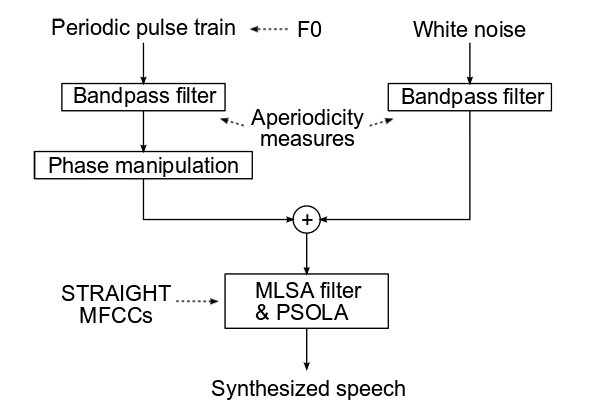
\includegraphics[width=0.6\textwidth]{images/straight_synthesis.jpg}
\caption{Block diagram of the synthesis process made by STRAIGHT \cite{manuMSc}}
\label{fig:straight_synthesis}
\end{centering}
\end{figure}

The components for the mixed excitation are generated by sub-band filtering the voice and unvoiced parts, impulse train and white Gaussian noise respectively, in a separate way in the frequency domain.

The band-pass filters used are determined by the aperiodicity coefficients, having the resultant sub-bands the same average lower-to-upper envelope ratio as the correspondent aperiodicity coefficient.

The pulse train component is all-pass filtered to adjust the phase characteristics of the excitation.

The synthesis quality of STRAIGHT has a mean opinion score (MOS) of 3, while the impulse excitation vocoder (see \ref{vocoders_basics}) obtains a MOS of 2.